\begin{picture}(0,0)%
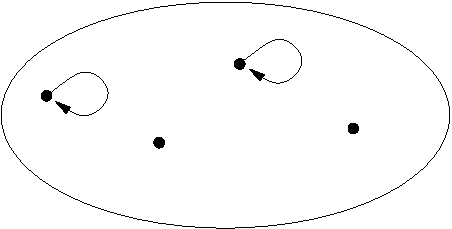
\includegraphics{./vacuously_symmetric.pdf}%
\end{picture}%
\setlength{\unitlength}{3947sp}%
%
\begingroup\makeatletter\ifx\SetFigFont\undefined%
\gdef\SetFigFont#1#2#3#4#5{%
  \reset@font\fontsize{#1}{#2pt}%
  \fontfamily{#3}\fontseries{#4}\fontshape{#5}%
  \selectfont}%
\fi\endgroup%
\begin{picture}(3606,1822)(1653,-1801)
\put(1824,-774){\makebox(0,0)[lb]{\smash{{\SetFigFont{12}{14.4}{\familydefault}{\mddefault}{\updefault}{\color[rgb]{0,0,0}a}%
}}}}
\put(2701,-1186){\makebox(0,0)[lb]{\smash{{\SetFigFont{12}{14.4}{\familydefault}{\mddefault}{\updefault}{\color[rgb]{0,0,0}b}%
}}}}
\put(3376,-511){\makebox(0,0)[lb]{\smash{{\SetFigFont{12}{14.4}{\familydefault}{\mddefault}{\updefault}{\color[rgb]{0,0,0}c}%
}}}}
\put(4276,-1036){\makebox(0,0)[lb]{\smash{{\SetFigFont{12}{14.4}{\familydefault}{\mddefault}{\updefault}{\color[rgb]{0,0,0}d}%
}}}}
\end{picture}%
